\chapter{Mise en oeuvre et tests du module d'extension \texttt{qtype\_essayhelper}}
Le site de Moodle donne une br\`eve introduction \`a la cr\'eation d'un nouveau type de question \footnote{\url{https://docs.moodle.org/dev/Question\_types\#Question\_type\_plug\_in\_development}}.
Un gabarit est disponible afin d'aider \`a d\'ebuter, mais le site conseille de modifier ou copier un type de question existant s'il est similaire au type de question que l'on d\'esire d\'evelopper.
Dans notre cas, nous allons utiliser le type de question \texttt{qtype\_essay} comme base, car il poss\`ede presque toutes les fonctionnalit\'es d\'esir\'ees.
Les commentaires de \emph{copyrights} ont \'et\'e ajust\'es comme illustr\'e \`a l'exemple de code~\ref{code:commentaire}.
\begin{lstfloat}
\begin{lstlisting}[frame=l]
/**
 * Essay for correction helper question definition class.
 *
 * @package    qtype
 * @subpackage essayhelper
 * @copyright  2018 Philippe Girard
 * @license    http://www.gnu.org/copyleft/gpl.html GNU GPL v3 or later
 *
 * Inspired by:
 * @package    qtype
 * @subpackage essay
 * @copyright  2009 The Open University
 * @license    http://www.gnu.org/copyleft/gpl.html GNU GPL v3 or later
 */
\end{lstlisting}
\caption{Exemple des commentaires dans les fichiers du module d'extension.}
\label{code:commentaire}
\end{lstfloat}
\section{Fonctionnalit\'es du module d'extension \texttt{qtype\_essayhelper}}
Pour obtenir notre nouveau module d'extension,
certaines fonctionnalit\'es du module d'extension \texttt{qtype\_essay} ont \'et\'e enlev\'ees, notamment les suivantes:
\begin{description}
  \item[\'Editeur de texte WYSIWIG]
  
  Cet \'editeur permet de modifier facilement l'apparence du texte.
  Ceci permet, entre autres, de surligner, de souligner, de mettre en gras, de mettre en italique et plus encore.
  Comme on ne peut pas enlever des options WYSIWIG pour un seul module d'extension, cela devient complexe de trouver une mise en forme qui permet de mettre en \'evidence les mots cl\'es, car un \'etudiant pourrait, par erreur, reproduire la m\^eme mise en forme.
  
  \item[Remise de fichier]
  
  Il est possible d'\'ecrire directement dans la zone de texte ou de remettre un document texte (configurable par l'enseignant).
  Comme le module d'extension n'aidera pas \`a corriger les textes remis par fichier, cette option a \'et\'e enlev\'ee.
\end{description}
Plusieurs fonctionnalit\'es ont \'et\'e conserv\'ees dans le nouveau module d'extension:
\begin{description}
  \item[R\'etroaction g\'en\'erale]
  
  Cette fonctionnalit\'e permet de laisser un commentaire \`a l'\'etudiant une fois que la correction est termin\'ee.
  Par exemple, l'enseignant pourrait laisser des explications sur les erreurs courantes.
  
  \item[Mod\`ele de r\'eponse]
  
  Ceci permet de pr\'eremplir la zone de texte de l'\'etudiant avec le texte donn\'e.
  Par exemple, un en-t\^ete de fonction pour une question de programmation ou la liste des mots \`a d\'efinir.
  
  \item[Information de l'\'evaluateur]
  
  Ceci affiche un texte pour le correcteur seulement.
  Utile pour voir facilement le bar\`eme de correction ou donner des instructions au correcteur.
  Cette information est affich\'ee sous la r\'eponse de l'\'etudiant lors de la correction.
\end{description}
Finalement, les fonctionnalit\'es suivantes ont \'et\'e ajout\'ees:
\begin{description}
  \item[Mots-cl\'es]
  
  Les mots-cl\'es sont mis en \'evidence dans la r\'eponse de l'\'etudiant lors de la correction manuelle.
  
  \item[R\'eponse officielle de l'enseignant]
  
  Cette r\'eponse de l'enseignant est 
  affich\'ee \`a droite de la r\'eponse de l'\'etudiant lors de la correction, et
  les mots-cl\'es sont aussi mis en \'evidence.
  
  \item[Langue de racination]
  
  La librairie \texttt{php-stemmer} supporte plusieurs langues.
  Toutes ces langues sont disponibles lors de la cr\'eation de la question.
\end{description}
\section{Structure des fichiers pour le module d'extension \texttt{qtype\_essayhelper}}
\begin{figure}[htbp]
   \begin{center}
  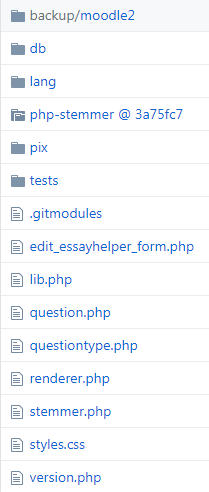
\includegraphics[scale=1]{images/architecture.png}
  \end{center}
  \caption{Structure des fichiers du module d'extension \texttt{qtype\_essayhelper} \GT{\`a compl\'eter!}.}
  \label{dev-architecture}
\end{figure}
L'installation d'un module d'extension dans Moodle est relativement simple.
Premi\`erement, il faut mettre le r\'epertoire du module d'extension au bon endroit.
Par exemple, un type de question doit se trouver dans le dossier \og question/type \fg{}.
Deuxi\`emement, il faut se connecter sur Moodle en tant qu'administrateur.
Moodle d\'etectera automatiquement qu'il y a un nouveau module d'extension.
Finalement, Moodle proposera \`a l'administrateur d'installer le nouveau module d'extension avant que l'administrateur puisse acc\'eder au syst\`eme.
\`A l'int\'erieur du r\'epertoire du module d'extension, chaque fichier doit avoir le bon nom et \^etre au bon endroit.
La structure du code est illustr\'ee \`a la figure \ref{dev-architecture} et d\'ecrite ci-dessous.
 
\begin{description}
 \item[backup/moodle2]
 Fichier qui g\`ere la sauvegarde et la restauration des questions de ce type.
 Le sous-dossier moodle2 indique que cette fonctionnalit\'e existe seulement pour la version 2 de Moodle et les suivantes.
 
 \item[db]
 
 Contient un fichier \texttt{install.xml} qui d\'efinit la table de base de donn\'ees \`a cr\'eer pour ce module d'extension.
 
 \item[lang]
 
 Contient un sous-dossier par langue support\'ee sois \og fr \fg{} et \og en \fg{} dans ce projet.
 Chaque sous-dossier contient un fichier PHP qui d\'efinit les cha\^ines de traduction.
 Ce dossier de traduction est valide pour les fonctionnalit\'es Moodle, pas pour la racination.
 
 \item[php-stemmer]
 
 Sous-module git pour ce projet uniquement.
 Pointe vers la biblioth\`eque de racination utilis\'ee,  d\'ecrite \`a la section~\ref{chap:phpstemmer}.
 
 \item[pix]
 
 Contient l'ic\^one du type de question.
 Cette ic\^one est uniquement visible lorsque l'enseignant choisit le type de question pour une nouvelle question.
 
 \item[tests]
 
 Ce dossier contient tous les tests unitaires et d'acception du module d'extension.
 Pour plus de d\'etail, voir la section \ref{dev_test}.
 
 \item[edit\_essayhelper\_form.php]
 
 D\'efinit le formulaire que l'enseignant remplit lorsqu'il cr\'e une question de ce type.
 Il faut uniquement d\'efinir les champs sp\'ecifiques au type de question actuel, Moodle ajoute automatiquement les champs de base comme le nom de la question et la valeur (points) de la question dans le questionnaire.
 
 \item[question.php]
 
 G\`ere la r\'eponse \`a une question.
 D\'efinit le comportement de question \`a utiliser, comment afficher la r\'eponse (appel renderer.php) et valide la pr\'esence d'une r\'eponse.
 
 \item[questiontype.php]
 
 G\`ere la cr\'eation, modification et suppression d'une question de ce type.
 
 \item[renderer.php]
 
 G\`ere l'affichage d'une question et des r\'eponses.
 Permet de contr\^oler la zone de texte pour une nouvelle r\'eponse ou pour la modifier.
 Permet aussi de changer l'affichage de la r\'eponse pour le correcteur.
 C'est principalement dans ce fichier que nous allons travailler.
 
 \item[stemmer.php]
 
 Fichier sp\'ecialement con\c{c}u pour ce module d'extension.
 C'est dans ce fichier que nous g\'erons le lien entre Moodle et \texttt{php-stemmer}.
 
 \item[styles.css]
 
 Fichier css pour notre module d'extension.
 
 \item[version.php]
 
 Fichier contenant quatre informations:
 \begin{itemize}
   \item \texttt{component}: 
   Nom du module d'extension qui sera utilis\'e dans la base de donn\'ees Moodle.
   Dans ce projet il s'agit de \texttt{qtype\_essayhelper}.
   
   \item \texttt{version}:
   Num\'ero de version du module d'extension dans le format \og aaaammjj00 \fg{} utilisant la date.
   Les deux derniers \og 0 \fg{} sont utilis\'es pour faire plus qu'une version par jour.
   Pour que Moodle prenne en compte les changements au fichier \texttt{install.xml} (pour la base de donn\'ees), il faut changer le num\'ero de version.
   
   \item \texttt{requires}:
   Num\'ero de version Moodle n\'ecessaire au bon fonctionnement du module d'extension utilisant aussi le format \og aaaammjj00 \fg{}.
   Notre module d'extension utilise la m\^eme d\'ependance que \texttt{qtype\_essay}, soit \og 2015111600 \fg{} qui repr\'esente Moodle 3.0.
   
   \item \texttt{maturity}:
   La maturit\'e du module d'extension.
   Notre module d'extension se trouve encore en \texttt{MATURITY\_ALPHA}.
 \end{itemize}
\end{description}
Dans tous les fichiers, nous avons d\^u adapter un peu le code afin de passer de \texttt{qtype\_essay} \`a \texttt{qtype\_essayhelper}.
\section{Les classes du module \texttt{qtype\_essayhelper}}
Le code du module d'extension est peu complexe.
Ce qui cause de la complexit\'e dans le projet r\'eside dans l'interaction entre le coeur de Moodle et ces classes.
La figure~\ref{dev-class} illustre les diff\'erentes classes qui seront d\'etaill\'ees dans les prochaines pages.
\begin{landscape}
\begin{figure}[htbp]
  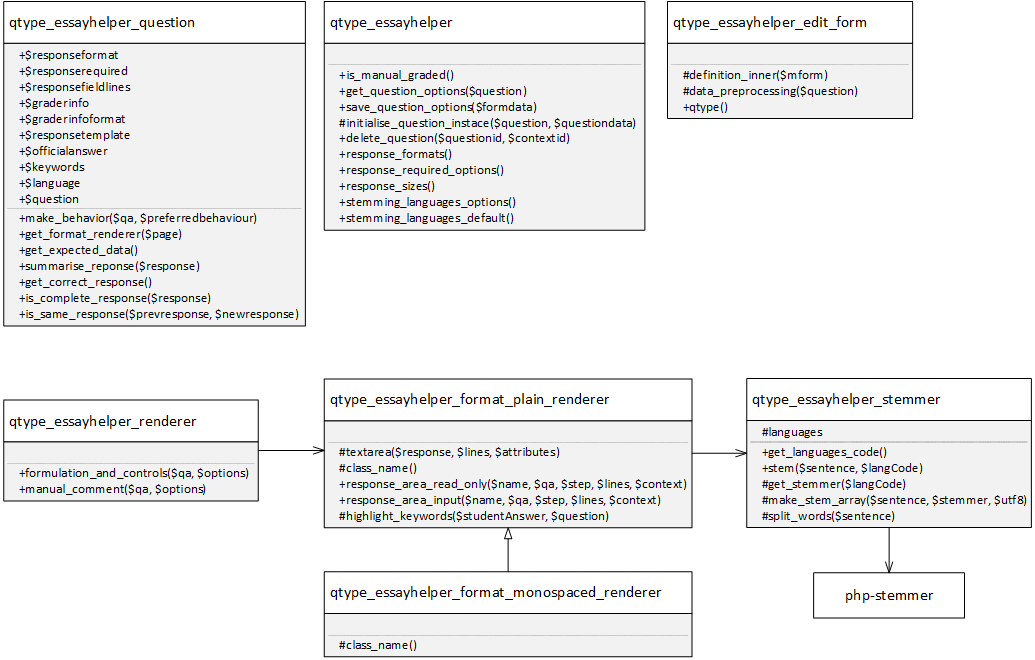
\includegraphics[scale=0.77]{images/class.png}
  \caption{Les principales classes associ\'ees au module \texttt{qtype\_essayhelper}.}
  \label{dev-class}
\end{figure}
\end{landscape}
\GT{Les noms d'identificateur dans le texte, de m\^eme que les
extraits de code, devraient \^etre mis en police \texttt{texttt}.}
\subsection*{Classe \texttt{qtype\_essayhelper\_edit\_form}}
Cette classe g\`ere le formulaire de cr\'eation et modification de question pour ce type de question.
Elle poss\`ede deux fonctions, la premi\`ere est \texttt{definition\_inner} qui permet d'ajouter des champs au formulaire de base de cr\'eation de questions.
Le formulaire de base comporte quelques champs tels que le titre de la question, le texte de la question ainsi que le nombre de points que vaut cette question.
La gestion des champs de base se fait automatiquement par Moodle, il ne reste donc qu'\`a ajouter les champs suppl\'ementaires pour notre type de question.
L'ajout de champs se fait avec un objet formulaire fourni par Moodle.
L'exemple de code~\ref{code:formdefinition} illustre l'ajout des champs d'aide \`a la correction dans le formulaire de notre module d'extension.
La fonction principale de cet objet est \texttt{addElement} qui prend quatre param\`etres:
\begin{enumerate}
  \item Le type d'\'el\'ement;
  \item Le nom du champ, qui doit \^etre le m\^eme que dans la base de donn\'ees;
  \item Le texte \`a afficher, la fonction \texttt{get\_string} traduit la cha\^ine donn\'ee en premier param\`etre dans les fichiers de traductions du module d'extension donn\'e dans le deuxi\`eme param\`etre;
  \item Si n\'ecessaire, des options suppl\'ementaires.
\end{enumerate}
\begin{lstfloat}
\begin{lstlisting}[frame=l]
$qtype = question_bank::get_qtype('essayhelper');
$mform->addElement('header', 'essayhelper', get_string('essayhelperheader', 'qtype_essayhelper'));
$mform->setExpanded('essayhelper');
$mform->addElement('textarea', 'officialanswer', get_string('officialanswer', 'qtype_essayhelper'),
 array('rows' => 10, 'cols' => 100));
$mform->addElement('textarea', 'keywords', get_string('keywords', 'qtype_essayhelper'),
 array('rows' => 10, 'cols' => 60));
$mform->addHelpButton('keywords', 'keywords', 'qtype_essayhelper');
\end{lstlisting}
\caption{Extrait du code de la fonction \texttt{definition\_inner} de la classe \texttt{qtype\_essayhelper\_edit\_form}.}
\label{code:formdefinition}
\end{lstfloat}
La deuxi\`eme fonction de cette classe permet de sauvegarder les champs du formulaire.
Tous les champs non reconnus par Moodle doivent \^etre trait\'es manuellement dans cette fonction comme illustr\'ee \`a l'exemple de code \ref{code:formpreprocessing}.
\begin{lstfloat}
\begin{lstlisting}[frame=l]
$question->responsetemplate = $question->options->responsetemplate;
$question->officialanswer = $question->options->officialanswer;
$question->keywords = $question->options->keywords;
\end{lstlisting}
\caption{Extrait du code de la fonction \texttt{data\_preprocessing} de la classe \texttt{qtype\_essayhelper\_edit\_form}.}
\label{code:formpreprocessing}
\end{lstfloat}
\subsection*{Classe \texttt{qtype\_essayhelper\_question}}
Cette classe g\`ere la r\'eponse \`a une question, que ce soit pour une nouvelle r\'eponse, une modification de r\'eponse ou afficher la r\'eponse au correcteur.
Les fonctions d\'efinies dans cette classe sont les suivantes:
\begin{description}
  \item[\texttt{make\_behaviour}] Retourne le comportement utilis\'e par le type de question. \texttt{manualgraded} dans ce cas.
  \item[\texttt{get\_format\_renderer}] Retourne la classe \texttt{qtype\_essayhelper\_renderer} qui s'occupera de l'affichage de la question.
  \item[\texttt{get\_expected\_data}] Retourne ce que la r\'eponse de l'\'etudiant doit contenir. Dans notre cas, il y a seulement une r\'eponse textuelle.
  \item[\texttt{summarise\_response}] Retourne un r\'esum\'e de la r\'eponse de l'\'etudiant, dans notre cas il s'agit de la r\'eponse directement. Elle est utilis\'ee dans les modules de correction afin de donner un aper\c{c}u de la r\'eponse de chaque \'etudiant.
  \item[\texttt{get\_correct\_response}] Devrait retourner la bonne r\'eponse \`a la question. Notre fonction retourne \texttt{null} afin d'indiquer \`a Moodle qu'il n'y a pas de bonne r\'eponse.
  \item[\texttt{is\_complete\_response}] V\'erifie si l'\'etudiant a r\'epondu \`a la question. Nous v\'erifions simplement s'il y a une r\'eponse non-vide.
  \item[\texttt{is\_same\_response}] D\'etermine si l'\'etudiant a modifi\'e sa r\'eponse.
\end{description}
\subsection*{Classe \texttt{qtype\_essayhelper}}
Cette classe g\`ere les options du type de question ainsi que les interactions \`a la base de donn\'ees.
Les fonctions d'interactions avec la base de donn\'ees sont les suivantes:
\begin{description}
  \item[\texttt{is\_manual\_graded}] Retourne \texttt{vrai} dans notre cas pour indiquer que la question doit se corriger manuellement.
  \item[\texttt{get\_question\_options}] R\'ecup\`ere les options pour la question d\'efinie dans la base de donn\'ees. Nous retournons simplement le r\'esultat de la requ\^ete.
  \item[\texttt{save\_question\_options}] Ici, il faut prendre les donn\'ees du formulaire et les ajouter dans la base de donn\'ees. G\`ere la cr\'eation et la modification de la question.
  \item[\texttt{initialise\_question\_instance}] Initialise l'instance de la question en ajoutant les options \`a l'objet repr\'esentant la question.
  \item[\texttt{delete\_question}] Supprime la question de la base de donn\'ees. Notre type de question n'utilise qu'une seule table, il s'agit donc d'une seule requ\^ete \texttt{DELETE}.
\end{description}
Les options du type de question sont des listes d\'eroulantes dans le formulaire de cr\'eation et modification de question.
Les fonctions qui d\'efinissent les options sont les suivantes:
\begin{description}
  \item[\texttt{response\_formats}] Retourne les formats de r\'eponses possibles soit \og Texte pur \fg{} et \og Texte pur, police monospace \fg{} .
  \item[\texttt{response\_required\_options}] Retourne deux options soit \og Requiert la saisie d'un texte par le participant \fg{} et \og Saisie de texte optionnelle \fg{}.
  \item[\texttt{response\_sizes}] Donne le nombre de lignes par d\'efaut que contiendra le champ de r\'eponse. Nous donnons les options de 5 \`a 40 avec des intervalles de 5.
  \item[\texttt{stemming\_languages\_options}] R\'ecup\`ere toutes les langues disponibles pour la racination et les traduit dans la langue de l'utilisateur avec la fonction \texttt{PHP Locale::getDisplayName}.
  \item[\texttt{stemming\_languages\_default}] Trouve la langue de racination par d\'efaut en se basant sur la langue actuelle de l'utilisateur. Si la langue n'est pas reconnue, l'anglais est utilis\'ee.
\end{description}
\subsection*{Classe \texttt{qtype\_essayhelper\_renderer}}
Cette classe g\`ere l'affichage de la question aux \'etudiants lorsqu'ils r\'epondent ainsi que l'affichage de la r\'eponse de l'\'etudiant lors de la relecture de celui-ci ou lors de la correction.
Elle ne contient que deux fonctions:
\begin{description}
  \item[\texttt{formulation\_and\_controls}] G\`ere l'affichage du texte de la question; la zone de r\'eponse de l'\'etudiant est g\'er\'ee par la classe \texttt{qtype\_essayhelper\_format\_}-\texttt{plain\_renderer}.
  \item[\texttt{manual\_comment}] G\`ere l'affichage de la zone de commentaire de l'enseignant lors de la correction. Pour chaque r\'eponse l'enseignant peut laisser un commentaire.
\end{description}
\subsection*{Classe \texttt{qtype\_essayhelper\_format\_plain\_renderer}}
Cette classe g\`ere la r\'eponse de l'\'etudiant.
\begin{description}
  \item[\texttt{textarea}] Fonction prot\'eg\'ee qui construit la zone de texte lorsqu'un \'etudiant r\'epond \`a la question.
  \item[\texttt{class\_name}] Fonction prot\'eg\'ee qui retourne le nom de la classe css \`a appliquer sur la balise \texttt{HTML} englobant la question et la r\'eponse.
  \item[\texttt{response\_area\_read\_only}] Fonction qui affiche le texte de la r\'eponse pour consultation seulement. Si c'est un enseignant ou un correcteur qui consulte la question dans le module de correction manuel on affiche la r\'eponse de l'enseignant \`a c\^ot\'e de la r\'eponse de l'\'etudiant et on met en \'evidence les mots cl\'es
  \item[\texttt{response\_area\_input}] Affiche la zone de texte cr\'e\'e par la fonction \texttt{textarea} afin que l'\'etudiant puisse r\'epondre \`a la question.
  \item[\texttt{highlight\_keywords}] Met en \'evidence les mots-cl\'es trouv\'es dans le texte par la racination.
\end{description}
La classe \texttt{qtype\_essayhelper\_format\_monospaced\_renderer} h\'erite de la classe \texttt{qtype\_essayhelper\_format\_plain\_renderer} et red\'efinit seulement la fonction \texttt{class\_name}.
Le CSS correspondant \`a la classe retourn\'ee est d\'efini dans le module d'extension \texttt{qtype\_essay}.
Un exemple de l'interaction de toutes ces classes avec Moodle est illustr\'e \`a la figure \ref{dev-diagramme}.
Cet exemple illustre l'ouverture d'un questionnaire par un \'etudiant.
\begin{landscape}
\begin{figure}[h!]
  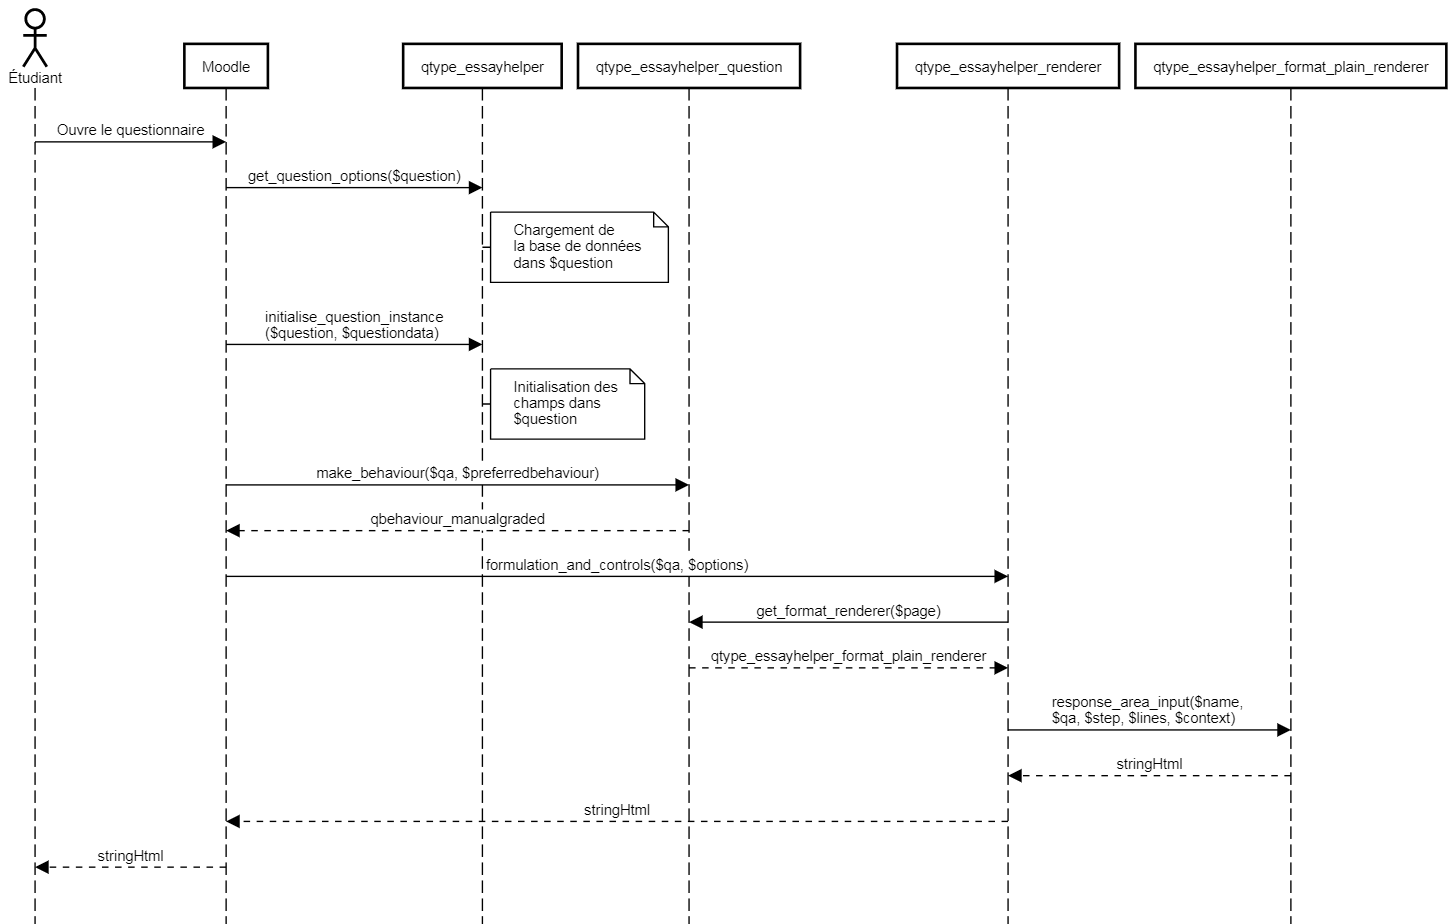
\includegraphics[scale=0.4]{images/diagramme-flux.png}
  \caption{Interaction entre Moodle et le module d'extension \texttt{qtype\_essayhelper}.}
  \label{dev-diagramme}
\end{figure}
\end{landscape}
\section{D\'etection des mots cl\'es}
Comme indiqu\'e dans le \autoref{chap:keywords}, nous utilisons la biblioth\`eque \texttt{php-stemmer} afin de trouver la racine de chaque mot.
Pour ce faire, il faut d\'ebuter par isoler chacun des mots du texte.
Les caract\`eres non alphanum\'eriques sont remplac\'es par des espaces et le texte est d\'ecoup\'e par les apostrophes et les caract\`eres d'espacement (espace, saut de ligne, tabulation, etc.) tel qu'illustr\'e dans l'extrait de code \ref{code:isoler}.
\begin{lstfloat}[htbp]
\begin{lstlisting}[frame=l]
$words = preg_split('/(\s|\')/', preg_replace('/[^[:alnum:][:space:]]/u', ' ', $sentence));
\end{lstlisting}
\caption{Isoler les mots du texte.}
\label{code:isoler}
\end{lstfloat}
Ensuite, chaque mot est associ\'e avec sa racine trouv\'ee avec l'algorithme Snowball tel qu'illustr\'e dans l'extrait de code \ref{code:racinationsnowball}.
Chaque mot-cl\'e a, pr\'ealablement, aussi \'et\'e r\'eduit \`a sa racine avec l'algorithme Snowball.
\begin{lstfloat}[htbp]
\begin{lstlisting}[language=php,frame=l]
foreach ($words as $word) {
 if ($word) {
  if (Wamania\Snowball\Utf8::check($word)) {
   $stem = $stemmer->stem($word);
   if (isset($stems[$stem])) {
    if (!in_array($word, $stems[$stem])) {
     $stems[$stem][] = $word;
    }
   } else {
    $stems[$stem] = array($word);
   }
  } else {
   $stems[] = $word;
  }
 }
}
\end{lstlisting}
\caption{Racination des mots avec Snowball.}
\label{code:racinationsnowball}
\end{lstfloat}
Finalement, les mots-cl\'es trouv\'es dans le texte sont mis en \'evidence, tel qu'illustr\'e dans l'extrait de code~\ref{code:mots-cles} et dans la figure \ref{dev-correction-screenshot}.
\begin{lstfloat}[htbp]
\begin{lstlisting}[language=php,frame=l]
$usedKeywords = array_intersect(array_keys($stems), $keywords);
foreach ($usedKeywords as $keyword) {
 $words = $answerWords[$keyword];
 foreach ($words as $word) {
  $studentAnswer = str_replace($word, '<b><u>' . $word . '</u></b>', $studentAnswer);
 }
}
\end{lstlisting}
\caption{Mise en \'evidence des mots-cl\'es trouv\'es.}
\label{code:mots-cles}
\end{lstfloat}
\begin{figure}[htbp]
  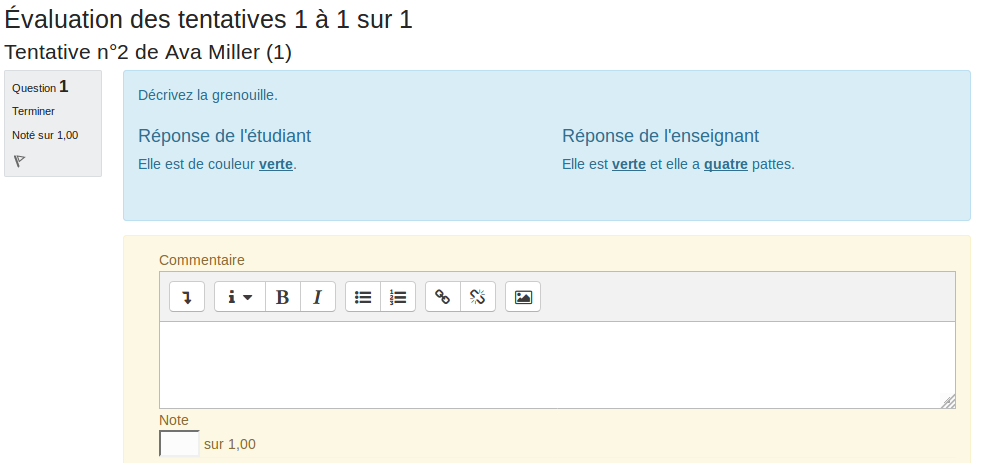
\includegraphics[scale=0.56]{images/correction-essayhelper.png}
  \caption{Mise en \'evidence des mots-cl\'es dans \texttt{qtype\_essayhelper}.}
  \label{dev-correction-screenshot}
\end{figure}
\section{Tests} \label{dev_test}
Les tests du module d'extension \texttt{qtype\_essay} ont \'et\'e conserv\'es et adapt\'es \`a notre nouveau module d'extension.
Par cons\'equent, le fonctionnement de base d'un module d'extension (cr\'eation de question, modification de question, r\'epondre \`a la question, etc.) a facilement \'et\'e test\'e.
Il ne restait donc plus qu'\`a tester les nouvelles fonctionnalit\'es de mots-cl\'es et d'affichage de la r\'eponse de l'enseignant.
\subsection{Tests d'acceptation} \label{dev_test_acceptation}
Un test d'acceptation a \'et\'e \'ecrit pour les nouvelles fonctionnalit\'es du module d'extension, le code est disponible \`a l'annexe~\ref{annexe_behat_new}, p.~\pageref{annexe_behat_new}.
Ce test v\'erifie qu'un enseignant peut voir l'aide \`a la correction (r\'eponse de l'enseignant et mots-cl\'es) mais qu'un \'etudiant n'y a pas acc\`es.
L'ex\'ecution de ce test avec \texttt{behat} confirme que les acc\`es fonctionnent correctement.

Les tests d'acceptation r\'ecup\'er\'es du module d'extension \texttt{qtype\_essay} ont permis de trouver quelques probl\`emes  dans le nouveau module d'extension.
Par exemple, la fonctionnalit\'e \textit{Backup and restore} ne fonctionnait pas pour les questions avec le nouveau type de question \texttt{qtype\_essayhelper}.
Le probl\`eme venait d'un dossier manquant dans le nouveau module.
Le dossier \textit{backup} dans le module d'extension \texttt{qtype\_essayhelper} ne contient pas de copies de sauvegarde du module d'extension, mais plusieurs versions de la fonctionnalit\'e \textit{Backup and restore}.

Une fois ce probl\`eme r\'esolu, les tests ont \'et\'e ex\'ectu\'es de nouveau. Six tests ont \'echou\'es, les m\^emes que d\'ecrits \`a la section \ref{test_acceptation}.
Les fonctionnalit\'es test\'es par ces tests ne n'impactent pas le module d'extension \texttt{qtype\_essayhelper}.
L'ajout de ce nouveau type de question n'\`a pas impact\'e le reste de Moodle selon les tests d'acceptation.
Les tests unitaires pourront confirmer le bon fonctionnement de Moodle.

\subsection{Tests unitaires} \label{dev_test_unitaire}
La biblioth\`eque de racination \texttt{php-stemmer} est d\'ej\`a test\'e unitairement et valid\'e \`a l'aide d'un dictionnaire qui associe les mots \`a leurs racines.
Il ne restait donc qu'\`a tester l'int\'egration entre Moodle et la biblioth\`eque de racination.
Cette int\'egration se retrouve dans la classe \texttt{qtype\_essayhelper\_stemmer} qui est test\'e dans la classe \texttt{qtype\_essayhelper\_stemmer\_test}.
Le code de cette derni\`ere se retrouve \`a l'annexe~\ref{annexe_unittest}, p.~\pageref{annexe_unittest}.
La classe \texttt{qtype\_essayhelper\_stemmer} comporte plusieurs fonctions prot\'eg\'ees qu'il faut tester, car chacune effectue un traitement important \`a la d\'etection de mots cl\'es.
Il faut donc utiliser la r\'eflexion \texttt{PHP} qui permet, entre autres, d'utiliser la fonction prot\'eg\'e ou priv\'e d'un objet.
La r\'eflexion ne modifie pas l'objet \`a l'ex\'ecution, mais permet de consulter son \'etat et ce qu'il contient (variables, constantes, classes h\'erit\'ees, interfaces impl\'ement\'ees, m\'ethodes, etc.).
Dans notre situation, la r\'eflexion cr\'ee un pointeur vers la fonction qui lui, est accessible.

Tous les tests Moodle ont \'et\'e ex\'ecut\'es \`a la fin du d\'eveloppement.
Il y avait une erreur de plus que celle d\'etect\'ee au d\'ebut et d\'ecrite au chapitre \ref{test-unitaires}, p.~\pageref{test-unitaires}.
Le nouveau test qui \'echoue compare la liste de module d'extension de base et compare \`a ceux qui sont pr\'esentement install\'es.
Comme il y a maintenant l'extension \texttt{qtype\_essayhelper} de plus le test \'echoue.

Comme les tests unitaires et d'acceptation de Moodle passent tous, le module d'extension \texttt{qtype\_essayhelper} ne r\'egresse pas les fonctionnalit\'es existantes de Moodle.